\documentclass{article}

% these packages let you do math
\usepackage{amsmath}
\usepackage{amssymb}

% we need these packages for fancy R tables
\usepackage{booktabs}
\usepackage{float}
\usepackage{colortbl}
\usepackage{xcolor}

% these packages play with the spacing/margins of the document. Uncomment the commands on lines 16 and 17 to see what they do.
\usepackage{a4wide}
\usepackage{setspace}
\usepackage{geometry}
\usepackage{parskip}
%\doublespacing
%\geometry{margin=1.5in}

% this package helps us with including images. Setting the graphics path makes it easier to refer to things in the \includegraphics command.
\usepackage{graphicx}
\graphicspath{ {../figures/} }

% make some hyperlinks using the \href command
\usepackage{hyperref}
\hypersetup{
    colorlinks=true,
    linkcolor=black,
    urlcolor=blue
}

% set the author, title, and date of the document. \maketitle adds it to the document.
\author{Elle Boodsakorn}
\title{My Paper on incarcerations Data}
\date{Sping 2022}

\begin{document}
\maketitle

\section{Introduction}

This paper analyzes incarceration data in 2002. The variable \texttt{incarcerated} is assigned to 1 if the person was incarcerated and 0 otherwise. Then, I calculate total incarcerations by race and gender. Section 2 presents a bar graph of total number of incarcerations in 2002 by race and gender, a table of total number of incarcerations, and a regression table.

\newpage

\section{Data}

Figure ~\ref{fig:graph} presents the total number of incarceration in 2002 categorized by race and gender. From the graph, we see that male were incarcerated a lot more than female for all race. Black male were incarcerated the most followed by Non-Black/Non-Hispanic and Hispanic respectively.


\begin{figure}[H]
    \begin{center}
        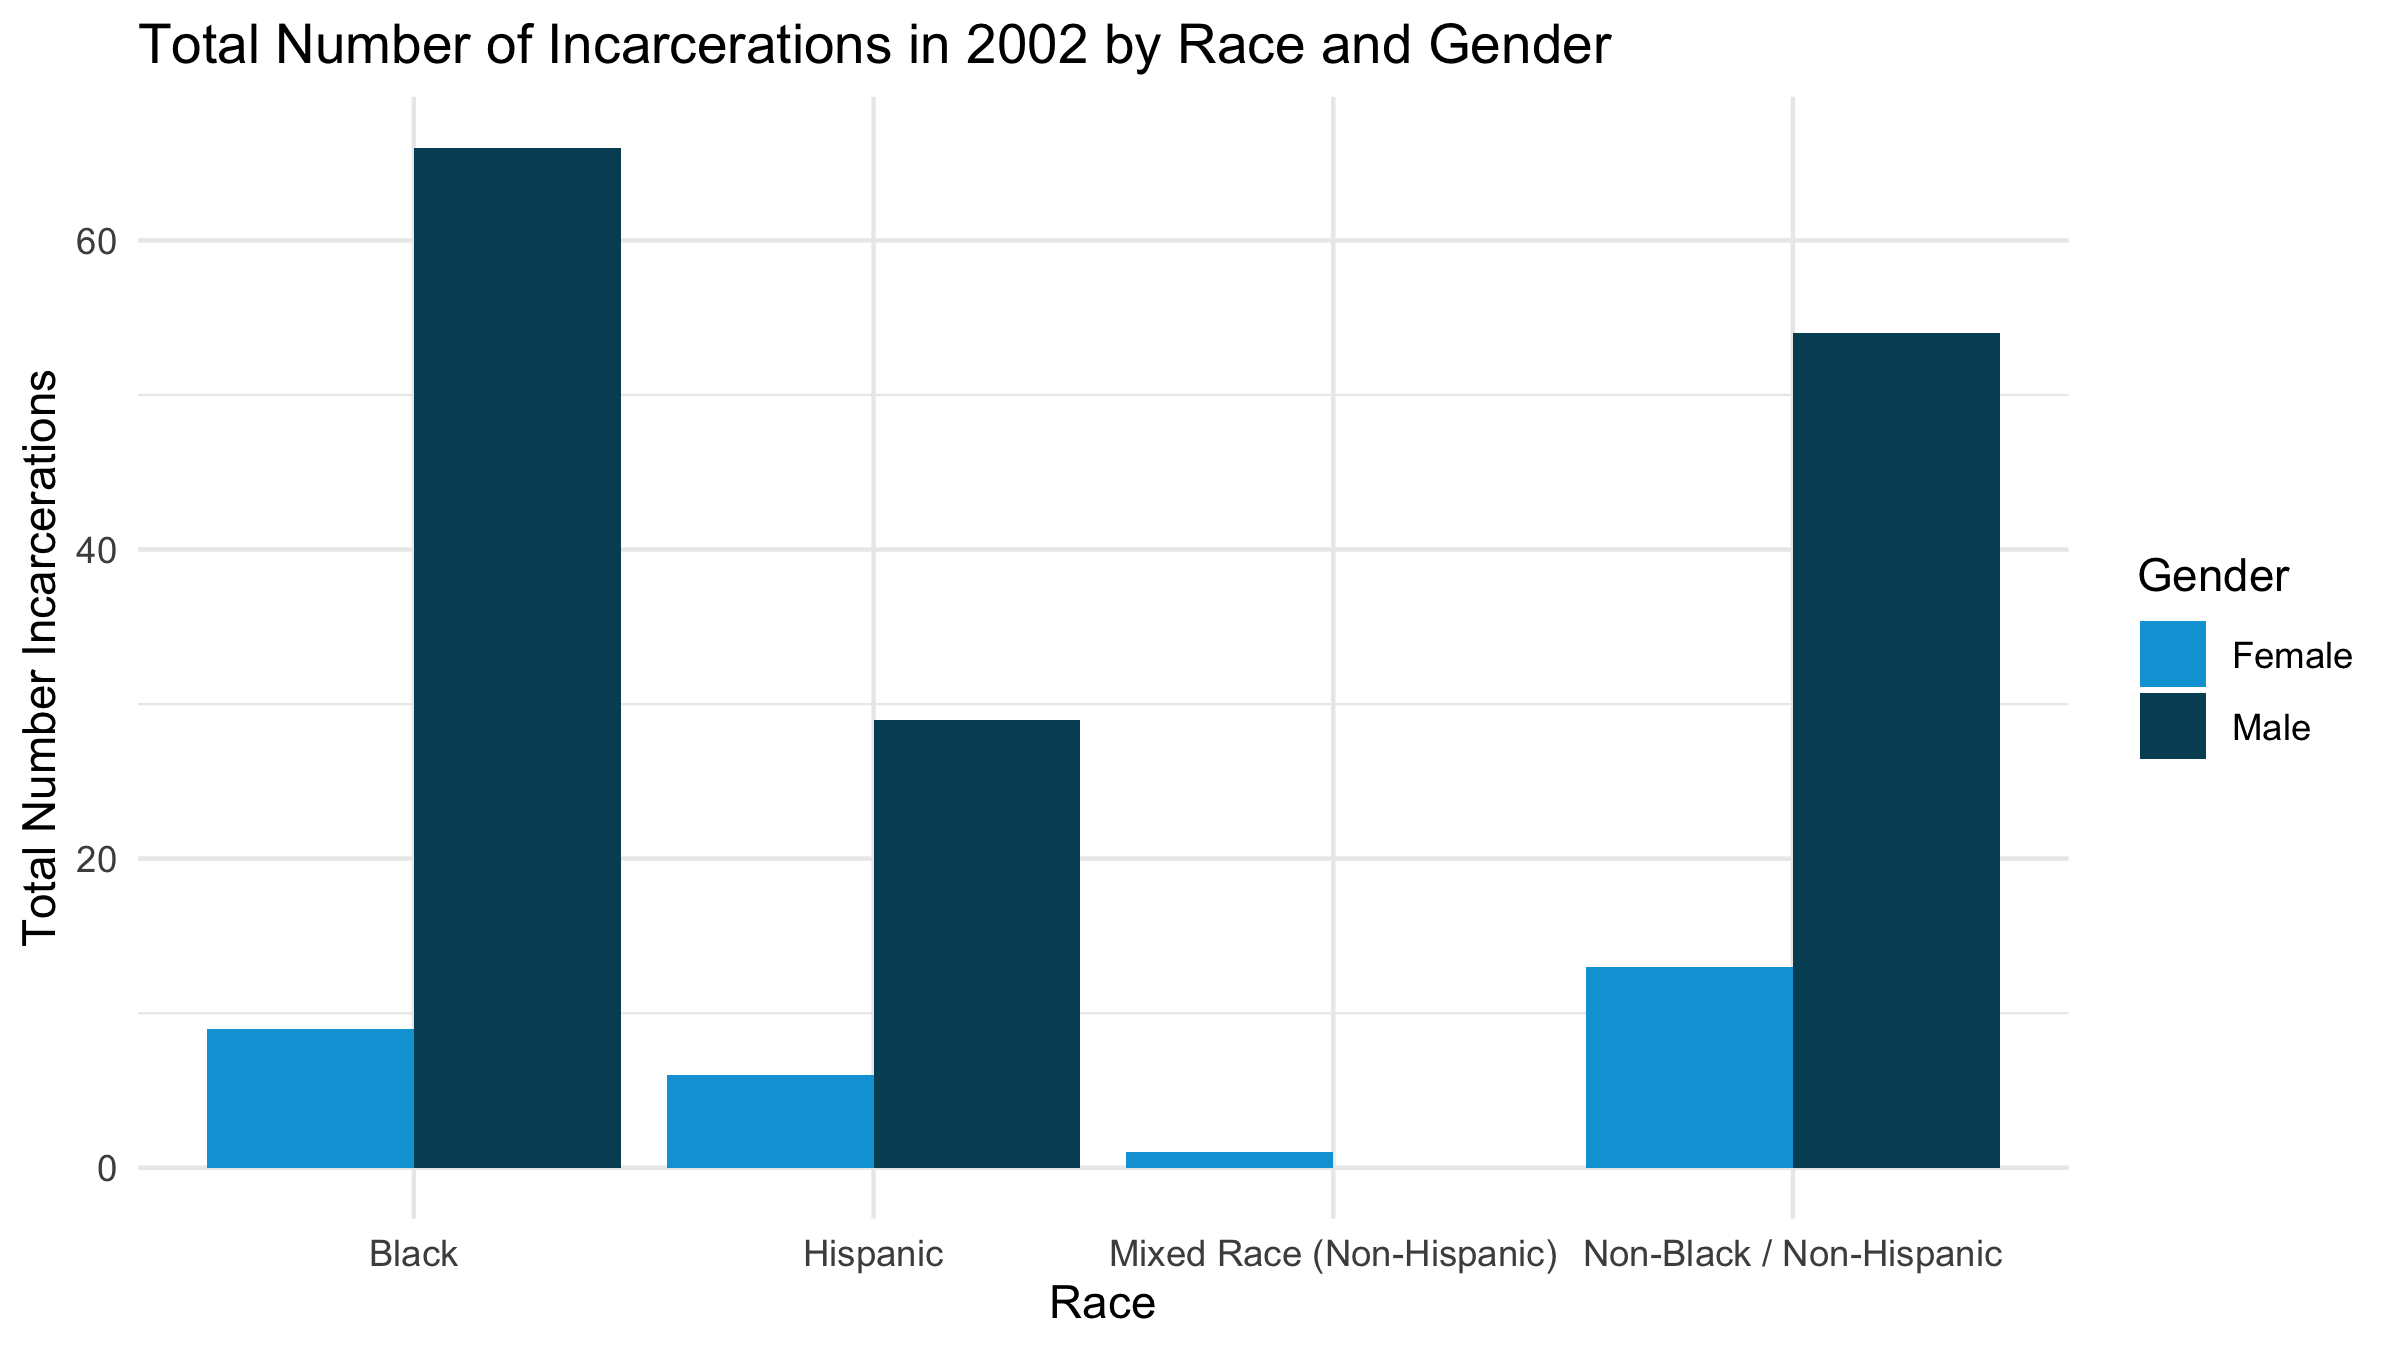
\includegraphics[width=.85\textwidth]{incarcerations_by_racegender}
    \end{center}
    \caption{Total Number of Incarceration in 2002 by Race and Gender}
    \label{fig:graph}
\end{figure}


The table below shows total number of incarcerations by race and gender.

\begin{table}[H]

\caption{\label{tab:tab:summarystats}Total number of incarcerations in 2002 by Race and Gender}
\centering
\begin{tabular}[t]{lrrrr}
\toprule
Gender & Black & Hispanic & Mixed Race Non Hispanic & Non Black Non Hispanic\\
\midrule
\cellcolor{gray!6}{Female} & \cellcolor{gray!6}{9} & \cellcolor{gray!6}{6} & \cellcolor{gray!6}{1} & \cellcolor{gray!6}{13}\\
Male & 66 & 29 & 0 & 54\\
\bottomrule
\end{tabular}
\end{table}


Table 2 presents the regression output regressing \texttt{incarcerations in 2002} on race and gender. The constant term reflects the probability of being incarcerated in 2002 for black female (base group). The coefficient -0.014 on Hispanic means that for female hispanic, the probability of being incarcerated is 1.4 percentage points lower than that of black female


% Table created by stargazer v.5.2.2 by Marek Hlavac, Harvard University. E-mail: hlavac at fas.harvard.edu
% Date and time: Wed, Feb 16, 2022 - 15:43:05
\begin{table}[!htbp] \centering 
  \caption{Regression Output. Omitted category is Black Females.} 
  \label{tab:regression} 
\begin{tabular}{@{\extracolsep{5pt}}lc} 
\\[-1.8ex]\hline 
\hline \\[-1.8ex] 
 & \multicolumn{1}{c}{\textit{Dependent variable:}} \\ 
\cline{2-2} 
\\[-1.8ex] & Incarcerations in 2002 \\ 
\hline \\[-1.8ex] 
 Hispanic & $-$0.014$^{***}$ \\ 
  & (0.005) \\ 
  & \\ 
 Mixed Race (Non-Hispanic) & $-$0.020 \\ 
  & (0.013) \\ 
  & \\ 
 Non-Black / Non-Hispanic & $-$0.018$^{***}$ \\ 
  & (0.004) \\ 
  & \\ 
 Male & 0.026$^{***}$ \\ 
  & (0.003) \\ 
  & \\ 
 Constant & 0.019$^{***}$ \\ 
  & (0.003) \\ 
  & \\ 
\hline \\[-1.8ex] 
Observations & 8,984 \\ 
R$^{2}$ & 0.012 \\ 
Adjusted R$^{2}$ & 0.011 \\ 
Residual Std. Error & 0.139 (df = 8979) \\ 
F Statistic & 26.252$^{***}$ (df = 4; 8979) \\ 
\hline 
\hline \\[-1.8ex] 
\textit{Note:}  & \multicolumn{1}{r}{$^{*}$p$<$0.1; $^{**}$p$<$0.05; $^{***}$p$<$0.01} \\ 
\end{tabular} 
\end{table} 


\end{document}
